\documentclass[conference,a4paper]{IEEEtran}
\usepackage[utf8]{inputenc}
\usepackage{booktabs}
\usepackage{enumitem} %resume enumerate
\usepackage{graphicx}
\usepackage{caption}
\usepackage{subcaption}
\usepackage{hyperref}
\usepackage{url}
\usepackage[x11names, svgnames, rgb]{xcolor}
\usepackage{tikz}
\usetikzlibrary{snakes,arrows,shapes}
\usepackage{amsmath}

\def\BibTeX{{\rm B\kern-.05em{\sc i\kern-.025em b}\kern-.08em
    T\kern-.1667em\lower.7ex\hbox{E}\kern-.125emX}}

\begin{document}

\title{Human Activity Recognition Using Smartphones}

\author{\IEEEauthorblockN{Roger Pujol}
\IEEEauthorblockA{\textit{Universitat Politècnica de Catalunya (UPC)}\\
Barcelona, Spain \\
roger.pujol.torramorell@est.fib.upc.edu}}

\date{\today}

\maketitle

\begin{abstract}
Nowadays everybody carries a smartphone and these devices are full of sensors. This includes accelerometers and gyroscopes, which could be used to get information about the activity of the person carrying it. In this paper we will use the information given by the sensors of a smartphone to recognize the activity done by the owner. Since this is a classification problem, we will use and analyse different methods in order to see which is the better for this particular case.\\
The code of this project is Open Source and can be found in: \url{https://github.com/rogerpt32/adm_paper3} \cite{code}.
\end{abstract}

\section{Introduction}
The smartphones have become probably the most used device for almost everybody. Furthermore everybody carries their smartphone everywhere they go and these devices are usually full of sensors. This makes the smartphone a perfect device to get data from people. In this paper we will use the data from the accelerometers and gyroscopes of a smartphone, in order to recognize what is doing the person carrying the device. Since this is a project for a Data Mining course, we will focus in testing several classification methods and comparing them for this particular data.

\section{Data Set}
The data set\cite{dataset} used in this paper is from the UCI Machine Learning Repository\cite{uci}. The experiments to extract the data have been carried out with a group of 30 volunteers within an age bracket of 19-48 years. Each person performed six activities (LAYING, SITTING, STANDING, WALKING, WALKING\_DOWNSTAIRS, WALKING\_UPSTAIRS) wearing a smartphone (Samsung Galaxy S II) on the waist. Using its embedded accelerometer and gyroscope, 3-axial linear acceleration and 3-axial angular velocity was captured at a constant rate of 50Hz. For each record in the data set it is provided:
\begin{itemize}
\item Triaxial acceleration from the accelerometer (total acceleration) and the estimated body acceleration.
\item Triaxial Angular velocity from the gyroscope.
\item A 561-feature vector with time and frequency domain variables.
\item Its activity label.
\item An identifier of the subject who carried out the experiment.
\end{itemize}
The activity label will obviously be our target to predict and we will remove the identifier since it shouldn't help to predict our target. We will randomly split the data in two parts, one for training the models which will have 75\% of the data, and another one for testing the accuracy which will have 25\% of the data.

\section{Experiments}
The implementation of the experiments has been done in Python 3 using mainly the Sklearn library and can be found in Github \cite{code}. 
\subsection{Gaussian Naive Bayes}
The first method we used is Gaussian Naive Bayes, which is quite straightforward, since it don't have any parameter to be tuned. This model gives us an 81.62\% in the testing part of the data set, which is quite good given the simplicity of the model. Taking a look at the confusion matrix (see Figure \ref{fig:cm_nb}), we can see that almost all the mispredictions are between the classes SITTING and STANDING, which is reasonable given the similarity of the classes, and between the multiple WALKING classes, which again intuitively are very similar.

\begin{figure}[htbp]
    \centering
    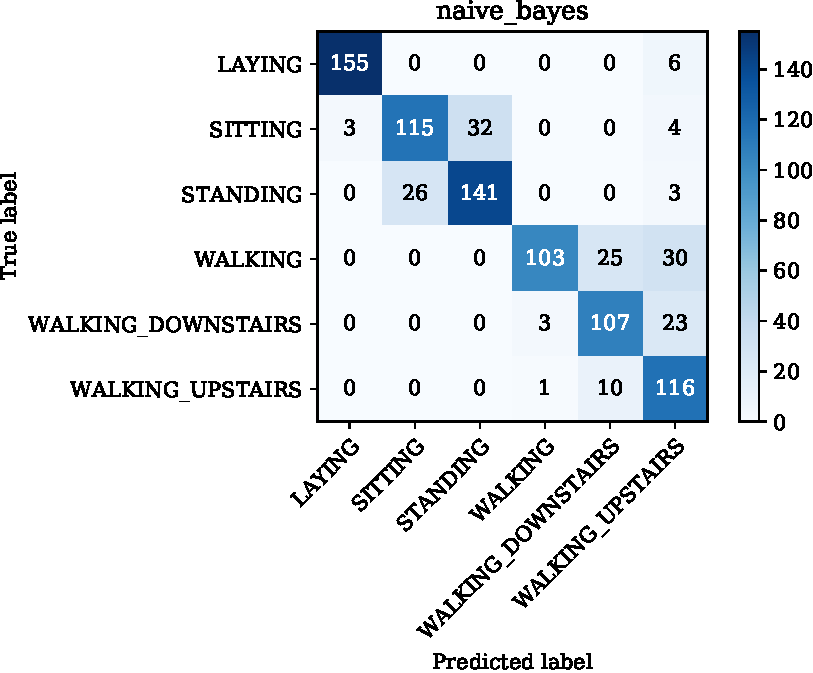
\includegraphics[width=0.8\columnwidth]{../plots/cm_naive_bayes.pdf}
    \caption{Confusion matrix of the Gaussian Naive Bayes model}
    \label{fig:cm_nb}
\end{figure}

\subsection{Decision Tree}
The second method we used is Decision Tree. In this method we have 2 main parameters to set: depth of the tree and the criterion for the nodes. \\
For the depth we can set it to an arbitrary number to limit the size of the final tree, or just let the tree grow enough until the input data is completely classified with 100\% accuracy. We tested this by limiting the depth to 5 and without limit and the results are almost equal (just a 2\% better without limit), then we choose to use the limited one because it will probably generalize better and with depth 5 we can even see (see Figure \ref{fig:dt}) the model and understand how it works. According to the generated tree, there are some features that are almost enough to detect an entire label (for example feature 56 to detect if the label is LAYING). \\
For the criterion we can use ``gini'' or ``entropy'' which will be the criterion used to choose which feature and threshold a new node is created. In our case there is almost no difference between criterions but ``gini'' has a very slight improvement in accuracy, for this reason we will use this criterion. \\
With the final model we have a testing accuracy of 87.71\%. Taking a look at the confusion matrix (see Figure \ref{fig:cm_dt}) we see almost the same errors from the previous classifier with a minor improvement.

\begin{figure}[htbp]
    \centering
    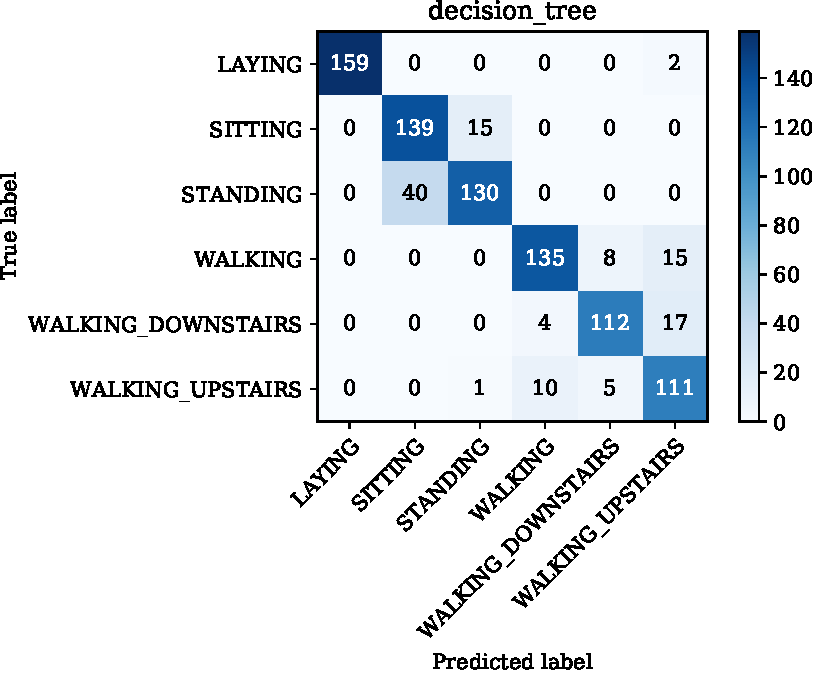
\includegraphics[width=0.8\columnwidth]{../plots/cm_decision_tree.pdf}
    \caption{Confusion matrix of the Decision Tree model}
    \label{fig:cm_dt}
\end{figure}

\subsection{Support Vector Machines (SVM)}
The third method we used is Support Vector Machines usually referred simply as SVM. This method is a bit more complex than the previous ones and have many things that can be tuned. For our problem we only tuned a few (kernel and the C parameter) since it wasn't worth to test more due to a very high accuracy. The kernels tested are:
\begin{itemize}
    \item RBF
    \item Poly (with degree 2, 3 and 4)
    \item Sigmoid
    \item Linear
\end{itemize}
And for each kernel we tested with a cost parameter (C parameter) of 1, 10, 100 and 1000. After some tests looks like for our data the bigger the C the better with improvements of up to 15\% in accuracy for C equal 100 or 1000, compared to C equal 1. With the different kernels, there is a tie in accuracy for RBF, Poly (degree 2) and Linear with around 97\% accuracy and Sigmoid is slightly worse. Since the Linear kernel is the simplest, its the one that we will use. Taking a look at the confusion matrix (see Figure \ref{fig:cm_svm}) we see almost no errors and again the conflicting classes are the ones we saw at the previous classifiers.

\begin{figure}[htbp]
    \centering
    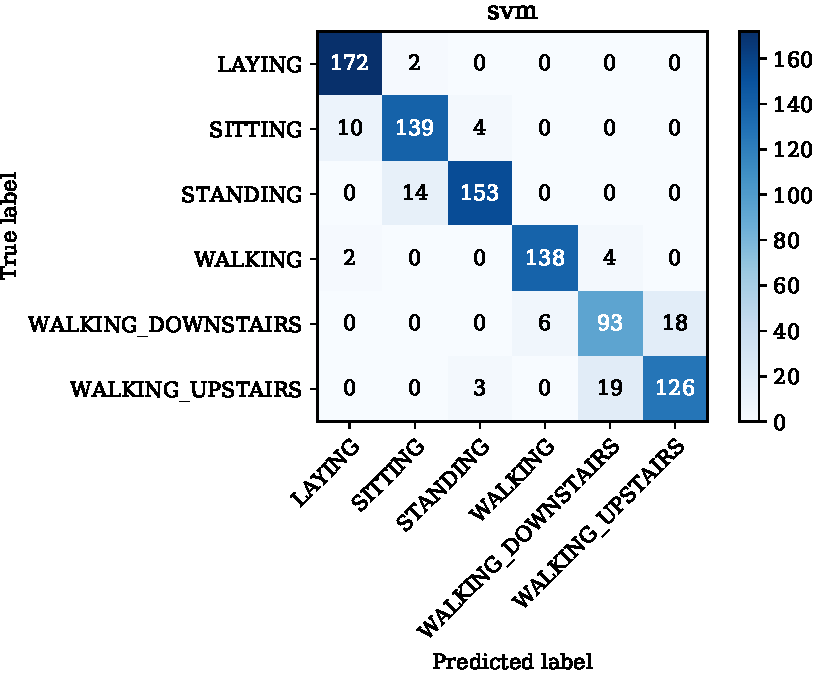
\includegraphics[width=0.8\columnwidth]{../plots/cm_svm.pdf}
    \caption{Confusion matrix of the Support Vector Machine model}
    \label{fig:cm_svm}
\end{figure}

\subsection{Multilayer Perceptron (MLP)}
The fourth method we used is a Multilayer Perceptron or MLP. This method is complex, requires a definition of the architecture of the network and some learning parameters. Since our data is quite simple to predict (seeing the results of the previous models), we tried to keep the architecture of the MLP as small as possible. The final results have only two hidden layers, the first with 12 nodes and the last one with 6 nodes. For the other learning parameters we only set them in a way to avoid early stops. The results have a 96.79\% accuracy in the test data. If we take a look at the confusion matrix (see Figure \ref{fig:cm_mlp}) we see almost the same results that we had with the SVM, with the only big difference being two misses from SITTING predicted as LAYING.

\begin{figure}[htbp]
    \centering
    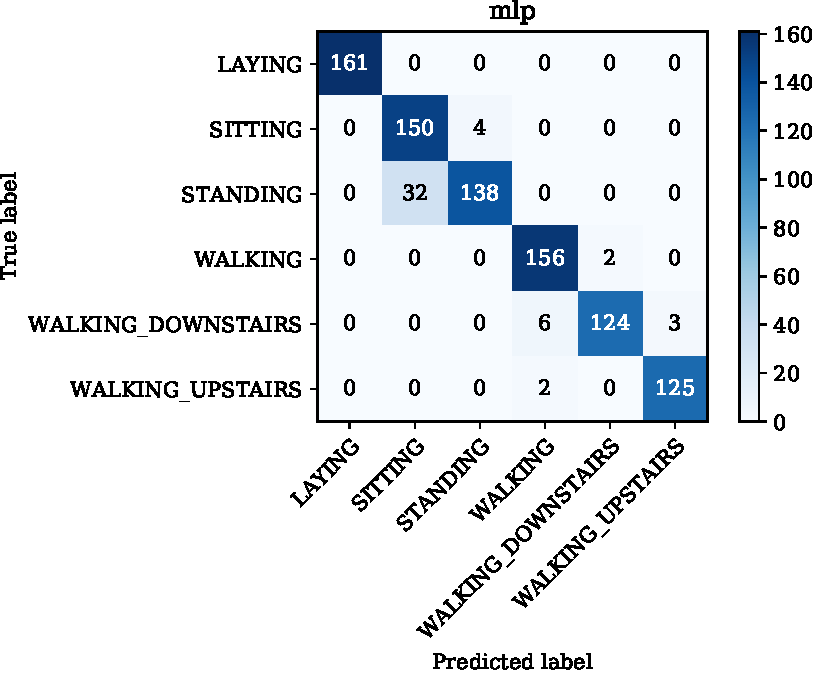
\includegraphics[width=0.8\columnwidth]{../plots/cm_mlp.pdf}
    \caption{Confusion matrix of the Multilayer Perceptron model}
    \label{fig:cm_mlp}
\end{figure}

\subsection{Random Forest}
The fifth method we used is Random Forest. This method basically uses multiple Decision Trees which are created with different conditions to finally predict using the average answer of all the trees. The parameters we tuned for this model are the same that we had in the single Decision Tree. Here to check the power of Random Forest we first tried with depth 5 to compare the result to the single Decision Tree, and the accuracy improved by around 2-3\%. Since its not much then we tried reducing the depth, and we see that using depth 4 we have almost the same accuracy than with a single Decision Tree. Finally we left the best which was the depth 5 which has an accuracy of 89.59\%. Taking a look at the confusion matrix (see Figure \ref{fig:cm_rf}) we can see that the results are almost the same that the ones from the single Decision Tree with a very slight improvement but with a small deterioration of the accuracy when predicting the SITTING class.

\begin{figure}[htbp]
    \centering
    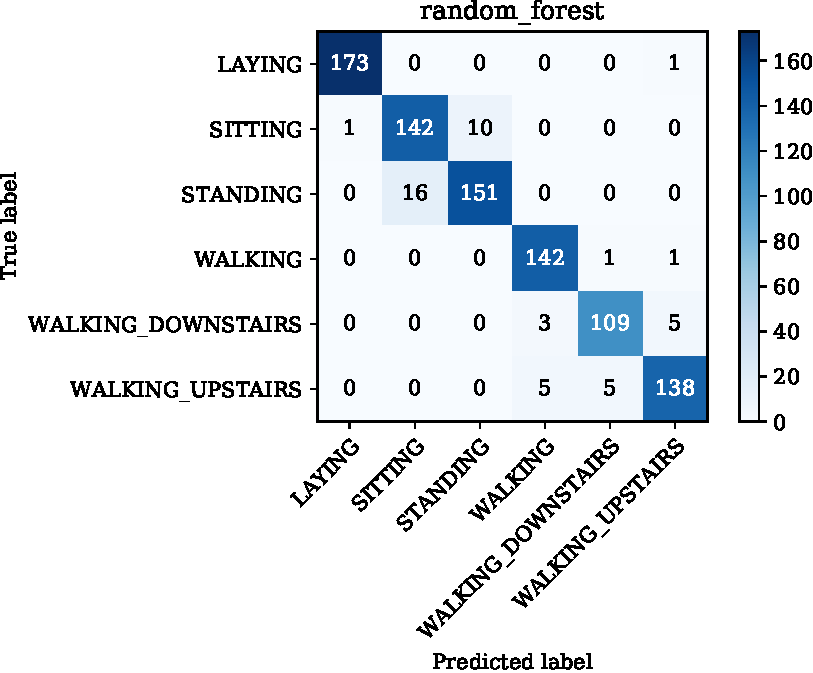
\includegraphics[width=0.8\columnwidth]{../plots/cm_random_forest.pdf}
    \caption{Confusion matrix of the Random Forest model}
    \label{fig:cm_rf}
\end{figure}

\subsection{AdaBoost}
Finally the last method we used is AdaBoost. This method takes a weak estimator and uses it multiplt times in order to get a strong estimator. As base estimators we tested Decision Trees with depth 1, 2 and 3 using a number of estimators inversly proportional to the depth size. Also we tested with Naive Bayes and SVM. \\
Naive Bayes almost don't have any difference and its logic given the way how Naive Bayes works. SVM is even worse than NB since its accuracy drops to 50\%, this two methods show which kind of estimators shouldn't be used as base estimators for AdaBoost because (as stated before) it works with weak estimators that can be improved by creating multiple of them. \\ 
\newpage
With the Decision Trees using small depth we create a weak estimators which the impact of different data might be relevant. Using depth 1 with 500 estimators, we have a very bad model which can only predict correctly some of the classes, probably because some classes are defined better with multiple features. Using depth 2 with 100 estimators, the accuracy improves a lot but still worse than all the models used before. Finally using depth 3 with 50 estimators we have a good model with a test accuracy of 92.25\%. Taking a look at the confusion matrix (see Figure \ref{fig:cm_ab}) we see the same distribution of errors of all the previous models.

\begin{figure}[htbp]
    \centering
    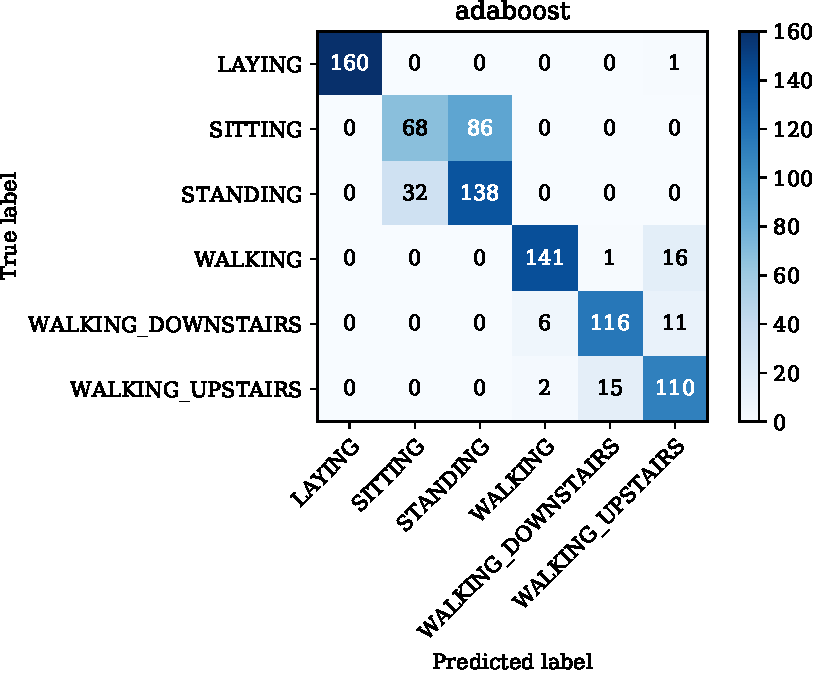
\includegraphics[width=0.8\columnwidth]{../plots/cm_adaboost.pdf}
    \caption{Confusion matrix of the AdaBoost model}
    \label{fig:cm_ab}
\end{figure}

\section{Conclusions}

All the methods tested could be ``acceptable'' for some applications since all of them have an accuracy above the 80\%. If we want the best classification we should rely on SVM or MLP methods since those gave accuracies above 95\% which is very high given that there are many features and not a lot of instances.

\bibliographystyle{unsrt}
\bibliography{cites}

\onecolumn
\appendix
\noindent\begin{minipage}{\textwidth}
    \centering
    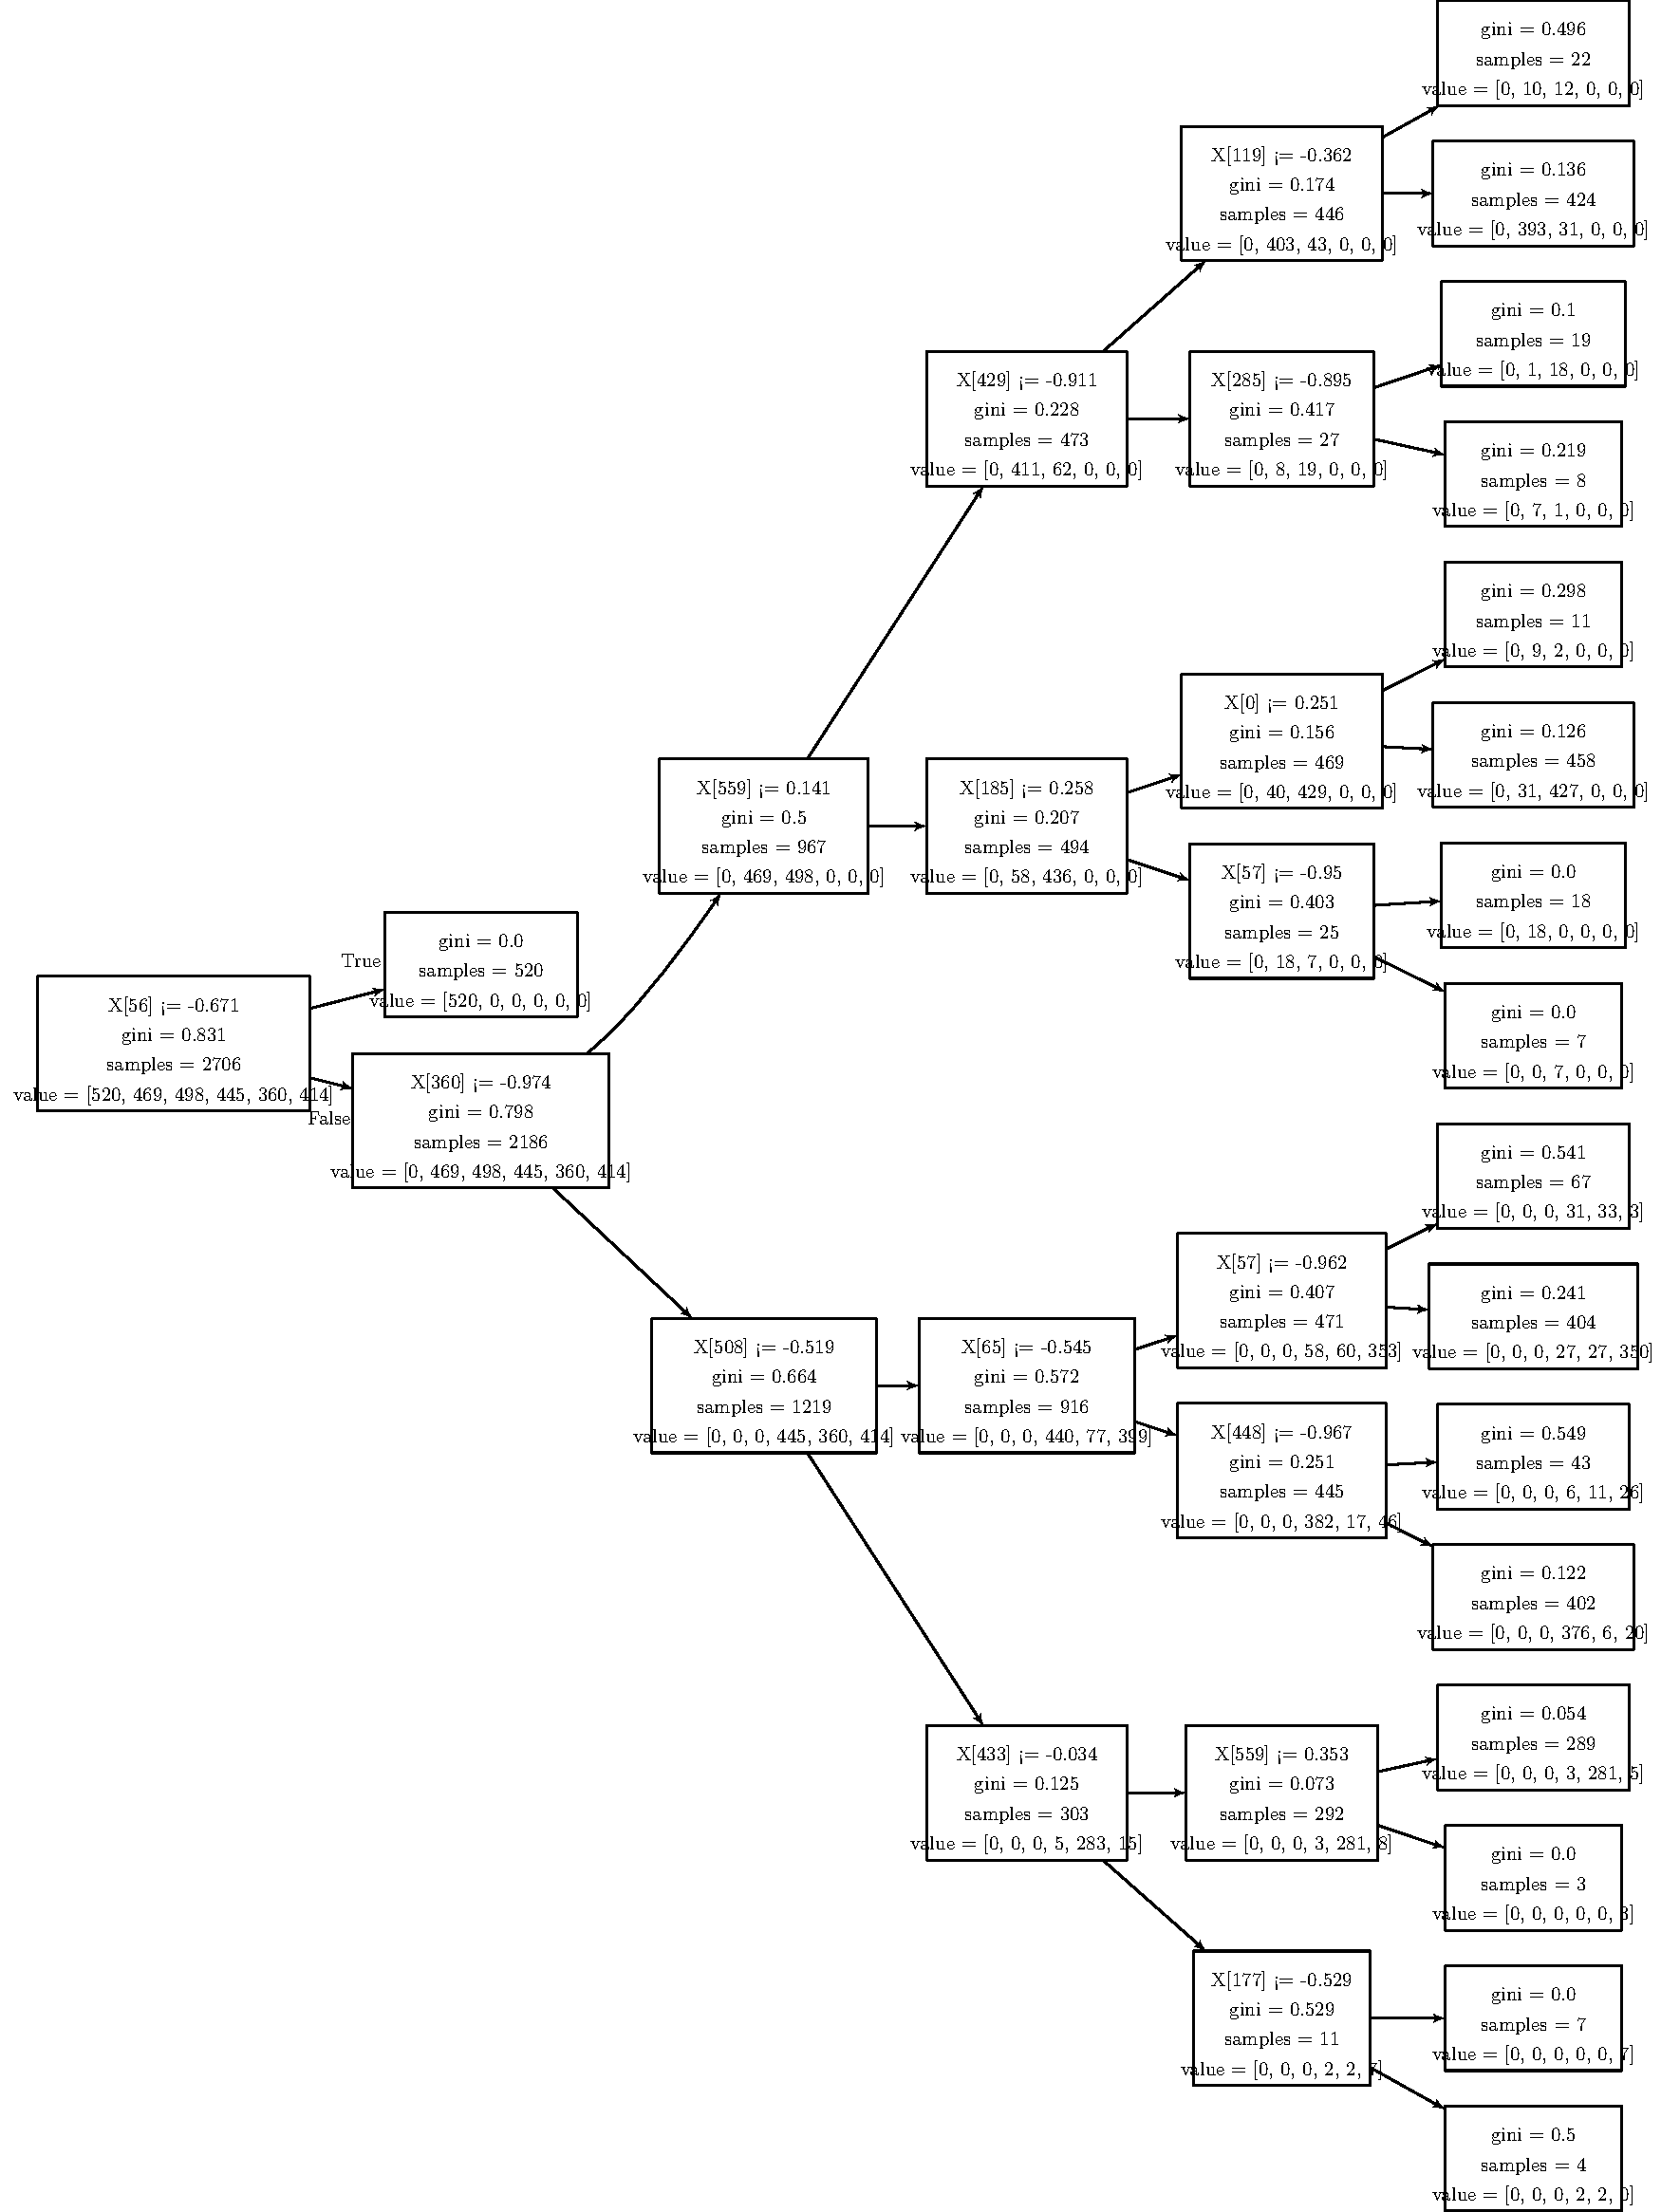
\includegraphics[width=0.93\linewidth]{decision_tree.pdf}
    \captionof{figure}{Full decision tree model}
    \label{fig:dt}
\end{minipage}

\end{document}